\documentclass{article}
\usepackage{amsfonts}
\usepackage{amstext}
\usepackage{pgfplots}
\pgfplotsset{compat = newest}

\title{Even solutions for Richard H. Hammack's Book of Proof}
\author{Martin Jaskulla}
\begin{document}
\maketitle
\section{Chapter}
\subsection{Section}
\paragraph{A.}
\begin{enumerate}
    \item [2] $\{3x+2:x \in \mathbb{Z} \} = \{...,-4,-1,2,5,8,...\}$
    \item [4] $\{x \in \mathbb{N}: -2 < x \leq 7 \} =\{1,2,3,4,5,6,7\}$
    \item [6] $\{x \in \mathbb{R}: x^2=9 \} =\{-3,3\}$
    \item [8] $\{x \in \mathbb{R}:x^3+5x^2=-6x \} =\{0,-2,-3\}$
    \item [10] $\{x \in \mathbb{R}: cos x = 1 \} =\{...,-2\pi,0,2\pi,...\}$
    \item [12] $\{x \in \mathbb{Z}: |2x|<5 \} =\{-2,-1,0,1,2\}$
    \item [14] $\{5x: x \in \mathbb{Z}, |2x| \leq8 \} =\{-20,-15,-10,-5,0,5,10,15,20\}$
    \item [16] $\{6a+2b: a,b \in \mathbb{Z} \} =\{...,-4,-2,0,2,4,...\}$
\end{enumerate}
\paragraph{B.}
\begin{enumerate}
    \item [18] $\{0,4,16,36,64,100,...\} = \{x^2: x \in \mathbb{W}, \text{x is even}\}$
    \item [20] $\{...,-8,-3,2,7,12,17,...\} = \{5x+2: x \in \mathbb{Z}\}$
    \item [22] $\{3,6,11,18,27,38,...\} = \{x^2+2:x\in \mathbb{Z}\}$
    \item [24] $\{-4,-3,-2,-1,0,1,2\} = \{ x: x\in \mathbb{Z}, -4 \leq x \leq 2\}$
    \item [26] $\{...,\frac{1}{27},\frac{1}{9},\frac{1}{3},1,3,9,27,...\} = \{ 3^x: x \in \mathbb{Z}\}$
    \item [28] $\{...,-\frac{3}{2},-\frac{3}{4},0,\frac{3}{4},\frac{3}{2},\frac{9}{4},3,\frac{15}{4},\frac{9}{2},...\} =\{x * \frac{3}{4}:x \in \mathbb{Z}\}$
\end{enumerate}
\paragraph{C.}
\begin{enumerate}
    \item [30] $|\{\{1,4\},a,b,\{\{3,4\}\},\{\emptyset\}\}| = 5$
    \item [32] $|\{\{\{1,4\},a,b,\{\{3,4\}\},\{\emptyset\}\}\}| = 1$
    \item [34] $|\{ x \in \mathbb{N}: |x|<10 \}| = 9$
    \item [36] $|\{ x \in \mathbb{N}: x^2<10 \}| = 3$
    \item [38] $|\{ x \in \mathbb{N}: 5x \le 20 \}| = 4$

\end{enumerate}
\paragraph{D.}
\begin{enumerate}
    \item [40] $\{(x,y):x \in [0,1], y\in [1,2] \}$ 
    \item []  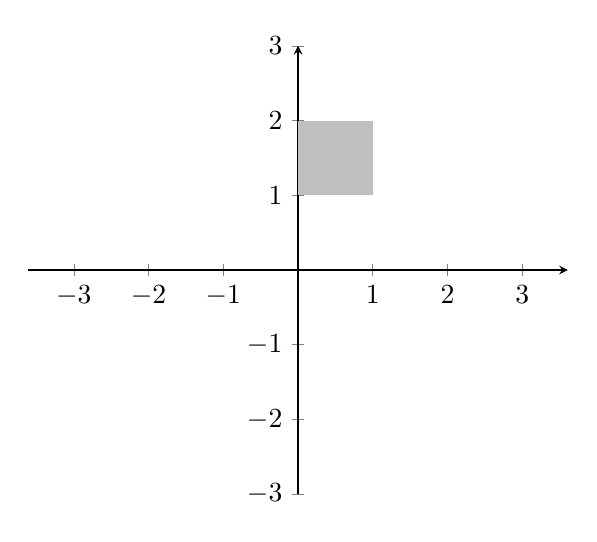
\begin{tikzpicture}
        \begin{axis}[
            axis lines=middle,
            axis equal,
            xmin=-3,
            xmax=3,
            ymin=-3,
            ymax=3,
            xtick={-3,...,3},
            ytick={-3,...,3}
            ]
            \fill[lightgray] (0,1) rectangle (1,2);
            \end{axis}
    \end{tikzpicture}
    \item [42] $\{(x,y):x = 2,y \in [0,1] \}$
    \item []  \begin{tikzpicture}
        \begin{axis}[
            axis lines=middle,
            axis equal,
            xmin=-3,
            xmax=3,
            ymin=-3,
            ymax=3,
            xtick={-3,...,3},
            ytick={-3,...,3}
            ]
            \draw[ultra thick] (2,0) -- (2,1);
            \end{axis}
    \end{tikzpicture}
    \item [44] $\{(x,x^2):x \in \mathbb{R} \} $
    \item []  \begin{tikzpicture}
        \begin{axis}[
            axis lines=middle,
            axis equal,
            xmin=-3,
            xmax=3,
            ymin=-3,
            ymax=3,
            xtick={-3,...,3},
            ytick={-3,...,3}
            ]
            \addplot[smooth] {x^2};
            \end{axis}
    \end{tikzpicture}
    \item [46] $\{(x,y):x,y \in \mathbb{R},x^2+y^2\leq1 \}$
    \item []  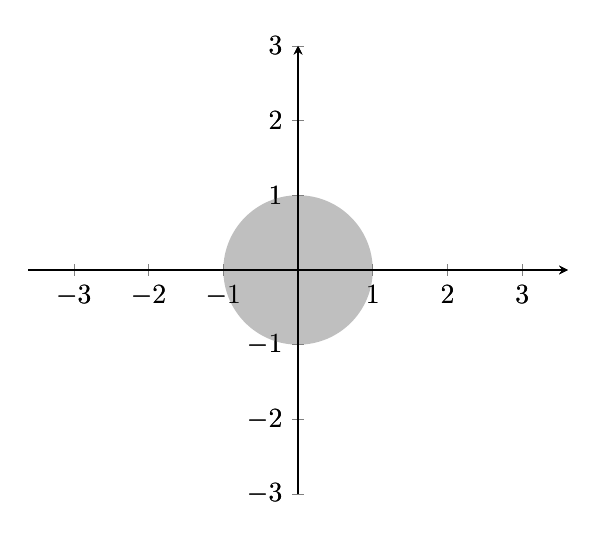
\begin{tikzpicture}
        \begin{axis}[
            axis lines=middle,
            axis equal,
            xmin=-3,
            xmax=3,
            ymin=-3,
            ymax=3,
            xtick={-3,...,3},
            ytick={-3,...,3}
            ]
            \fill[lightgray] (0,0) circle (1);
            \end{axis}
            \begin{axis}[
                axis lines=middle,
                axis equal,
                xmin=-3,
                xmax=3,
                ymin=-3,
                ymax=3,
                xtick={-3,...,3},
                ytick={-3,...,3}
                ]
                \end{axis}
    \end{tikzpicture}
    \item [48] $\{(x,y):x,y \in \mathbb{R},x > 1 \}$
    \item []  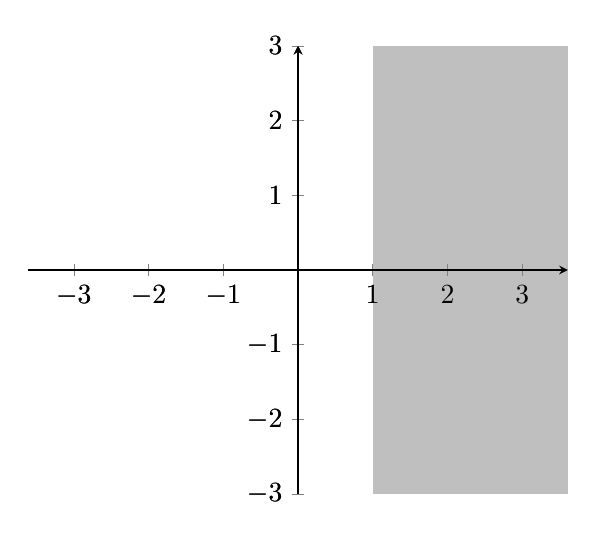
\begin{tikzpicture}
        \begin{axis}[
            axis lines=middle,
            axis equal,
            xmin=-3,
            xmax=3,
            ymin=-3,
            ymax=3,
            xtick={-3,...,3},
            ytick={-3,...,3}
            ]
            \fill[lightgray] (1,-3) rectangle(4,3);
            \end{axis}
            \begin{axis}[
                axis lines=middle,
                axis equal,
                xmin=-3,
                xmax=3,
                ymin=-3,
                ymax=3,
                xtick={-3,...,3},
                ytick={-3,...,3}
                ]
            \end{axis}
    \end{tikzpicture}
    \item [50] $\{(x,\frac{x^2}{y}):x \in \mathbb{R},y \in \mathbb{N} \}$
    \item []  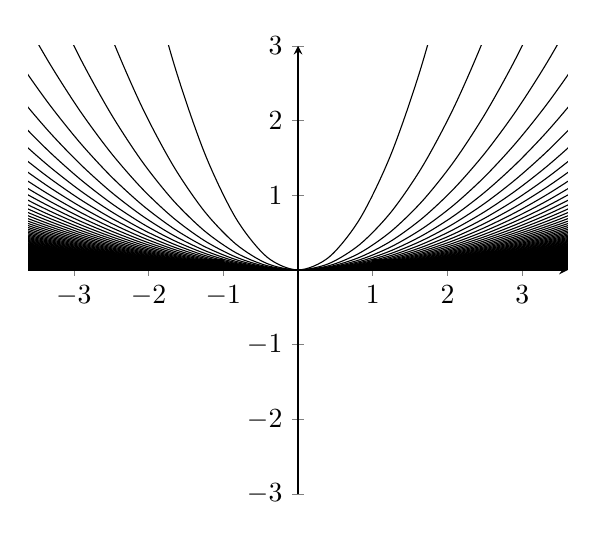
\begin{tikzpicture}
        \begin{axis}[
            axis lines=middle,
            axis equal,
            xmin=-3,
            xmax=3,
            ymin=-3,
            ymax=3,
            xtick={-3,...,3},
            ytick={-3,...,3}
            ]
            \foreach \i in {1,...,50}
            {
                \addplot[smooth] {x^2/\i};
            }
            \fill[] (1,0) rectangle(4,0.15);
            \fill[] (2.5,0) rectangle(4,0.25);
            \fill[] (-1,0) rectangle(-4,0.15);
            \fill[] (-2.5,0) rectangle(-4,0.25);
            \end{axis}
    \end{tikzpicture}
    \item [52] $\{(x,y) \in \mathbb{R}^2: (y-x^2)(y+x^2) =0 \}$
        \item []  \begin{tikzpicture}
        \begin{axis}[
            axis lines=middle,
            axis equal,
            xmin=-3,
            xmax=3,
            ymin=-3,
            ymax=3,
            xtick={-3,...,3},
            ytick={-3,...,3}
            ]
            \addplot[smooth] {x^2};
            \addplot[smooth] {-x^2};
            \end{axis}
    \end{tikzpicture}
\end{enumerate}

 
\end{document}

